\documentclass[11pt]{article}

\RequirePackage[l2tabu, orthodox]{nag}
%\documentclass{article}

\usepackage[left=1.25in, right=1.25in, top=1.25in, bottom=1.25in]{geometry}

% FONTS
%\usepackage[T1]{fontenc}

% Replace default Latin Modern typewriter with its proportional counterpart
% http://www.tug.dk/FontCatalogue/lmoderntypewriterprop/
%\renewcommand*\ttdefault{lmvtt}


%%% OPTION 1 - Fourier Math + New Century Schoolbook + ParaType Sans

% % Import Fourier Math (this imposes its own New Century Schoolbook type)
% % http://www.ctan.org/tex-archive/fonts/fouriernc/
%\usepackage{fouriernc}
%\usepackage{amsmath}
% % Replace with TeX Gyre Schola version of New Century Schoolbook (must scale!)
% % http://www.tug.dk/FontCatalogue/tgschola/
%\usepackage[scale=0.92]{tgschola}
%\usepackage[scaled=0.88]{PTSans}

%% OPTION 2 - MathDesign Math + Bitstream Charter + ParaType Sans

% Import MathDesign (this brings along Bitstream Charter)
% http://www.ctan.org/tex-archive/fonts/mathdesign/
\usepackage[bitstream-charter]{mathdesign}
 \usepackage{amsmath}
\usepackage[scaled=0.92]{PTSans}


% %%% OPTION 3 - MTPRO 2 Math + Termes Times + ParaType Sans

% \usepackage{tgtermes}
% \usepackage{amsmath}
% \usepackage[subscriptcorrection,
%             amssymbols,
%             mtpbb,
%             mtpcal,
%             nofontinfo  % suppresses all warnings
%            ]{mtpro2}
% \usepackage{scalefnt,letltxmacro}
% \LetLtxMacro{\oldtextsc}{\textsc}
% \renewcommand{\textsc}[1]{\oldtextsc{\scalefont{1.10}#1}}
% \usepackage[scaled=0.92]{PTSans}

% Use default fonts here
\usepackage{amsmath}
%\usepackage{amssymb}

% COLOR
\usepackage[usenames,dvipsnames]{xcolor}
\definecolor{shadecolor}{gray}{0.9}

% SPACING and TEXT
\usepackage[final,expansion=alltext]{microtype}
\usepackage[english]{babel}
\usepackage[parfill]{parskip}
\usepackage{afterpage}
\usepackage{framed}
\usepackage{verbatim}
\usepackage{setspace}

%redefine the leftbar environment to accept a width and coloring options
\renewenvironment{leftbar}[1][\hsize]
{%
  \def\FrameCommand
  {%
    {\color{Gray}\vrule width 3pt}%
    \hspace{10pt}%
    %\hspace{0pt}\fboxsep=\FrameSep\colorbox{black!10}%
  }%
  \MakeFramed{\hsize#1\advance\hsize-\width\FrameRestore}%
}%
{\endMakeFramed}

% define a paragraph header function
\DeclareRobustCommand{\parhead}[1]{\textbf{#1}~}

% EDITING
% line numbering in left margin
\usepackage{lineno}
\renewcommand\linenumberfont{\normalfont
                             \footnotesize
                             \sffamily
                             \color{SkyBlue}}
% ragged paragraphs in right margin
\usepackage{ragged2e}
\DeclareRobustCommand{\sidenote}[1]{\marginpar{
                                    \RaggedRight
                                    \textcolor{Plum}{\textsf{#1}}}}
% paragraph counter in right margin
\newcommand{\parnum}{\bfseries\P\arabic{parcount}}
\newcounter{parcount}
\newcommand\p{%
    \stepcounter{parcount}%
    \leavevmode\marginpar[\hfill\parnum]{\parnum}%
}
% paragraph helper
%\DeclareRobustCommand{\PP}{\textcolor{Plum}{\P} }

% COUNTERS
\usepackage[inline]{enumitem}
\renewcommand{\labelenumi}{\color{black!67}{\arabic{enumi}.}}
\renewcommand{\labelenumii}{{\color{black!67}(\alph{enumii})}}
\renewcommand{\labelitemi}{{\color{black!67}\textbullet}}

% FIGURES
\usepackage{graphicx}
\usepackage[labelfont={it, small}, font=small]{caption}
\usepackage[format=hang]{subcaption}

% APPENDIX FIGURES
\usepackage{chngcntr}

% TABLES
\usepackage{booktabs}

% ALGORITHMS
\usepackage[algoruled]{algorithm2e}
\usepackage{listings}
\usepackage{fancyvrb}
\fvset{fontsize=\normalsize}

% THEOREMS
\usepackage{amsthm}
\newtheorem{proposition}{Proposition}
\newtheorem{lemma}{Lemma}

% BIBLIOGRAPHY
\usepackage{natbib}

% HYPERREF
\usepackage[colorlinks,linktoc=all]{hyperref}
\usepackage[all]{hypcap}
\hypersetup{citecolor=MidnightBlue}
\hypersetup{linkcolor=MidnightBlue}
\hypersetup{urlcolor=MidnightBlue}

% CLEVEREF must come after HYPERREF
\usepackage[nameinlink]{cleveref}

% ACRONYMS
\usepackage[acronym,smallcaps,nowarn]{glossaries}
% \makeglossaries

% COLOR DEFINITIONS
\newcommand{\red}[1]{\textcolor{BrickRed}{#1}}
\newcommand{\orange}[1]{\textcolor{BurntOrange}{#1}}
\newcommand{\green}[1]{\textcolor{OliveGreen}{#1}}
\newcommand{\blue}[1]{\textcolor{MidnightBlue}{#1}}
\newcommand{\gray}[1]{\textcolor{black!60}{#1}}

% LISTINGS DEFINTIONS
\lstdefinestyle{mystyle}{
    commentstyle=\color{OliveGreen},
    keywordstyle=\color{BurntOrange},
    numberstyle=\tiny\color{black!60},
    stringstyle=\color{MidnightBlue},
    basicstyle=\ttfamily,
    breakatwhitespace=false,
    breaklines=true,
    captionpos=b,
    keepspaces=true,
    numbers=left,
    numbersep=5pt,
    showspaces=false,
    showstringspaces=false,
    showtabs=false,
    tabsize=2
}
\lstset{style=mystyle}

\usepackage[colorinlistoftodos,
            prependcaption,
            textsize=small,
            backgroundcolor=yellow,
            linecolor=lightgray,
            bordercolor=lightgray]{todonotes}

% !TEX root = template.tex

% \DeclareRobustCommand{\mb}[1]{\ensuremath{\boldsymbol{\mathbf{#1}}}}
\DeclareRobustCommand{\mb}[1]{\boldsymbol{#1}}

% \newcommand{\KL}[2]{\ensuremath{\textrm{KL}\PARENS{#1\;\|\;#2}}}
\DeclareRobustCommand{\KL}[2]{\ensuremath{\textrm{KL}\left(#1\;\|\;#2\right)}}

\DeclareMathOperator*{\argmax}{arg\,max}
\DeclareMathOperator*{\argmin}{arg\,min}

\renewcommand{\mid}{~\vert~}
\newcommand{\given}{\,|\,}
\newcommand{\iid}[1]{\stackrel{\text{iid}}{#1}}

\newcommand{\mba}{\mb{a}}
\newcommand{\mbb}{\mb{b}}
\newcommand{\mbc}{\mb{c}}
\newcommand{\mbd}{\mb{d}}
\newcommand{\mbe}{\mb{e}}
\newcommand{\mbg}{\mb{g}}
\newcommand{\mbh}{\mb{h}}
\newcommand{\mbi}{\mb{i}}
\newcommand{\mbj}{\mb{j}}
\newcommand{\mbk}{\mb{k}}
\newcommand{\mbl}{\mb{l}}
\newcommand{\mbm}{\mb{m}}
\newcommand{\mbn}{\mb{n}}
\newcommand{\mbo}{\mb{o}}
\newcommand{\mbp}{\mb{p}}
\newcommand{\mbq}{\mb{q}}
\newcommand{\mbr}{\mb{r}}
\newcommand{\mbs}{\mb{s}}
\newcommand{\mbt}{\mb{t}}
\newcommand{\mbu}{\mb{u}}
\newcommand{\mbv}{\mb{v}}
\newcommand{\mbw}{\mb{w}}
\newcommand{\mbx}{\mb{x}}
\newcommand{\mby}{\mb{y}}
\newcommand{\mbz}{\mb{z}}

\newcommand{\mbA}{\mb{A}}
\newcommand{\mbB}{\mb{B}}
\newcommand{\mbC}{\mb{C}}
\newcommand{\mbD}{\mb{D}}
\newcommand{\mbE}{\mb{E}}
\newcommand{\mbF}{\mb{F}}
\newcommand{\mbG}{\mb{G}}
\newcommand{\mbH}{\mb{H}}
\newcommand{\mbI}{\mb{I}}
\newcommand{\mbJ}{\mb{J}}
\newcommand{\mbK}{\mb{K}}
\newcommand{\mbL}{\mb{L}}
\newcommand{\mbM}{\mb{M}}
\newcommand{\mbN}{\mb{N}}
\newcommand{\mbO}{\mb{O}}
\newcommand{\mbP}{\mb{P}}
\newcommand{\mbQ}{\mb{Q}}
\newcommand{\mbR}{\mb{R}}
\newcommand{\mbS}{\mb{S}}
\newcommand{\mbT}{\mb{T}}
\newcommand{\mbU}{\mb{U}}
\newcommand{\mbV}{\mb{V}}
\newcommand{\mbW}{\mb{W}}
\newcommand{\mbX}{\mb{X}}
\newcommand{\mbY}{\mb{Y}}
\newcommand{\mbZ}{\mb{Z}}

\newcommand{\mbalpha}{\mb{\alpha}}
\newcommand{\mbbeta}{\mb{\beta}}
\newcommand{\mbdelta}{\mb{\delta}}
\newcommand{\mbepsilon}{\mb{\epsilon}}
\newcommand{\mbchi}{\mb{\chi}}
\newcommand{\mbeta}{\mb{\eta}}
\newcommand{\mbgamma}{\mb{\gamma}}
\newcommand{\mbiota}{\mb{\iota}}
\newcommand{\mbkappa}{\mb{\kappa}}
\newcommand{\mblambda}{\mb{\lambda}}
\newcommand{\mbmu}{\mb{\mu}}
\newcommand{\mbnu}{\mb{\nu}}
\newcommand{\mbomega}{\mb{\omega}}
\newcommand{\mbphi}{\mb{\phi}}
\newcommand{\mbpi}{\mb{\pi}}
\newcommand{\mbpsi}{\mb{\psi}}
\newcommand{\mbrho}{\mb{\rho}}
\newcommand{\mbsigma}{\mb{\sigma}}
\newcommand{\mbtau}{\mb{\tau}}
\newcommand{\mbtheta}{\mb{\theta}}
\newcommand{\mbupsilon}{\mb{\upsilon}}
\newcommand{\mbvarepsilon}{\mb{\varepsilon}}
\newcommand{\mbvarphi}{\mb{\varphi}}
\newcommand{\mbvartheta}{\mb{\vartheta}}
\newcommand{\mbvarrho}{\mb{\varrho}}
\newcommand{\mbxi}{\mb{\xi}}
\newcommand{\mbzeta}{\mb{\zeta}}

\newcommand{\mbDelta}{\mb{\Delta}}
\newcommand{\mbGamma}{\mb{\Gamma}}
\newcommand{\mbLambda}{\mb{\Lambda}}
\newcommand{\mbOmega}{\mb{\Omega}}
\newcommand{\mbPhi}{\mb{\Phi}}
\newcommand{\mbPi}{\mb{\Pi}}
\newcommand{\mbPsi}{\mb{\Psi}}
\newcommand{\mbSigma}{\mb{\Sigma}}
\newcommand{\mbTheta}{\mb{\Theta}}
\newcommand{\mbUpsilon}{\mb{\Upsilon}}
\newcommand{\mbXi}{\mb{\Xi}}

\newcommand{\dif}{\mathop{}\!\mathrm{d}}
\newcommand{\diag}{\textrm{diag}}
\newcommand{\supp}{\textrm{supp}}

\newcommand{\E}{\mathbb{E}}
\newcommand{\Var}{\mathbb{V}\textrm{ar}}
\newcommand{\bbH}{\mathbb{H}}
\newcommand{\bbI}{\mathbb{I}}
\newcommand{\bbN}{\mathbb{N}}
\newcommand{\bbZ}{\mathbb{Z}}
\newcommand{\bbR}{\mathbb{R}}
\newcommand{\bbS}{\mathbb{S}}

\newcommand{\cA}{\mathcal{A}}
\newcommand{\cB}{\mathcal{B}}
\newcommand{\cC}{\mathcal{C}}
\newcommand{\cD}{\mathcal{D}}
\newcommand{\cE}{\mathcal{E}}
\newcommand{\cF}{\mathcal{F}}
\newcommand{\cG}{\mathcal{G}}
\newcommand{\cH}{\mathcal{H}}
\newcommand{\cI}{\mathcal{I}}
\newcommand{\cJ}{\mathcal{J}}
\newcommand{\cK}{\mathcal{K}}
\newcommand{\cL}{\mathcal{L}}
\newcommand{\cM}{\mathcal{M}}
\newcommand{\cN}{\mathcal{N}}
\newcommand{\cO}{\mathcal{O}}
\newcommand{\cP}{\mathcal{P}}
\newcommand{\cQ}{\mathcal{Q}}
\newcommand{\cR}{\mathcal{R}}
\newcommand{\cS}{\mathcal{S}}
\newcommand{\cT}{\mathcal{T}}
\newcommand{\cU}{\mathcal{U}}
\newcommand{\cV}{\mathcal{V}}
\newcommand{\cW}{\mathcal{W}}
\newcommand{\cX}{\mathcal{X}}
\newcommand{\cY}{\mathcal{Y}}
\newcommand{\cZ}{\mathcal{Z}}

\newcommand{\trans}{\mathsf{T}}
\newcommand{\naturals}{\mathbb{N}}
\newcommand{\reals}{\mathbb{R}}

\newcommand{\distNormal}{\mathcal{N}}
\newcommand{\distGamma}{\mathrm{Gamma}}
\newcommand{\distBernoulli}{\mathrm{Bern}}
\newcommand{\distBinomial}{\mathrm{Bin}}
\newcommand{\distCategorical}{\mathrm{Cat}}
\newcommand{\distDirichlet}{\mathrm{Dir}}
\newcommand{\distMultinomial}{\mathrm{Mult}}
\newcommand{\distPolyaGamma}{\mathrm{PG}}
\newcommand{\distMNIW}{\mathrm{MNIW}}
\newcommand{\distPoissonProcess}{\mathrm{PP}}

\newcommand{\dtmax}{\Delta t_{\mathsf{max}}}

\newacronym{KL}{kl}{Kullback-Leibler}
\newacronym{ELBO}{elbo}{\emph{evidence lower bound}}
\newacronym{POPELBO}{pop-elbo}{\emph{population evidence lower bound}}

\newacronym{SVI}{svi}{stochastic variational inference}
\newacronym{BUMPVI}{bump-vi}{bumping variational inference}

\newacronym{GMM}{gmm}{Gaussian mixture model}
\newacronym{LDA}{lda}{latent Dirichlet allocation}

\newacronym{SUTVA}{sutva}{stable unit treatment value assumption}


\newcommand{\celegans}{\textit{C. elegans}}

% \title{\large Discrete and continuous latent states of neural activity in \textit{Caenorhabditis elegans}}
\title{Hierarchical recurrent models reveal latent states of neural activity in \textit{C. elegans}}
\author{Scott Linderman$^{\text{1}}$,
  Annika Nichols$^{\text{2}}$,
  David Blei$^{\text{1}}$,
  Manuel Zimmer$^{\text{2}}$,
  and
  Liam Paninski$^{\text{1}}$
  \\
  $^{\text{1}}$Columbia University,
  $^{\text{2}}$Research Institute of Molecular Pathology (IMP), Vienna Biocenter
}

\begin{document}

\doublespacing

\maketitle

\begin{abstract}
  Recent advances in neural recording technologies have enabled
  simultaneous measurements of the majority of head ganglia neurons in
  both immobilized and freely-behaving
  \celegans~\citep{schrodel2013brain, prevedel2014simultaneous,
    nguyen2016whole}.  The dynamics of neural activity shed light on
  how \celegans~processes sensory information and generates motor
  activity.  To understand these dynamics, we develop recurrent state
  space models that decompose complex time-series into segments with
  simple, linear dynamics. We incorporate these models into a robust,
  hierarchical framework for combining information across whole-brain
  recordings of many worms.  Using this framework, we reveal latent
  states of population neural activity, along with the discrete
  behavioral modes that drive dynamics in this latent state space.  We
  find stochastic transition patterns between these discrete
  behavioral modes, and we see that transition probabilities are
  determined by a combination of current brain state and environmental
  cues.  In addition to quantifying neural dynamics, this
  probabilistic framework aids in neural identification---currently a
  laborious, manual task---and reveals clusters of neurons that are
  similarly tuned in latent state space.  Finally, we find a
  significant overlap between our inferred states and the
  manually-labeled states of~\citet{kato2015global}
  and~\citet{nichols2017global}, which were shown to correspond to
  different behaviors, like forward crawling, reversals, and
  turns. Our methods automatically discover and quantify these
  behaviorally-meaningful states directly from neural activity,
  yielding powerful new tools for neuro-behavioral analysis.
\end{abstract}

\clearpage

\section*{Introduction}

\clearpage

\section*{Results}

\subsection*{A probabilistic framework that combines information across
  trials to learn canonical dynamics}

We seek a parsimonious characterization of the dynamics of neural
activity in the head ganglia of \celegans. Recent advances in optical
imaging offer simultaneous recordings of most of the head ganglia
neurons, but we must surmount three main challenges in order to learn
a dynamics model from these data.  First, we need to design a model
flexible enough to capture nonlinear dynamics yet interpretable enough
to reveal simplifying structure when it exists.  Moreover, any model
will necessarily be an approximation to the true neural dynamics, and
as such we need to be robust to data that does not quite match model
predictions.  Finally, our model must combine partial recordings from
separate organisms to learn shared neural dynamics yet still allow for
individual variability. We construct a recurrent, robust, and
hierarchical state space model that addresses these challenges,
decomposing complex dynamics into a collection of simpler pieces that
can be learned from noisy, partial recordings with trial-to-trial
variability.

We study the data presented in~\citet{kato2015global} and
\citet{nichols2017global}, which consist of a collection of optical
recordings of calcium fluorescence in immobilized \celegans. The
recordings are 18 minutes long with a frame rate of about 3Hz.  On
average, about 100 single units are extracted from each
recording. \celegans~is genetically stereotyped and each of its 302
neurons has a unique label (e.g. \textsf{AVAL}). On average, 30 single
units could be unambiguously labeled in each
recording. Fig.~\ref{fig:model}a illustrates this type of data. The
three panels represent recordings from three separate worms, and the
rows correspond to different neuron labels.  Neural activity is
measured for only a subset of neurons in each worm.

\begin{figure}[t!]
\centering%
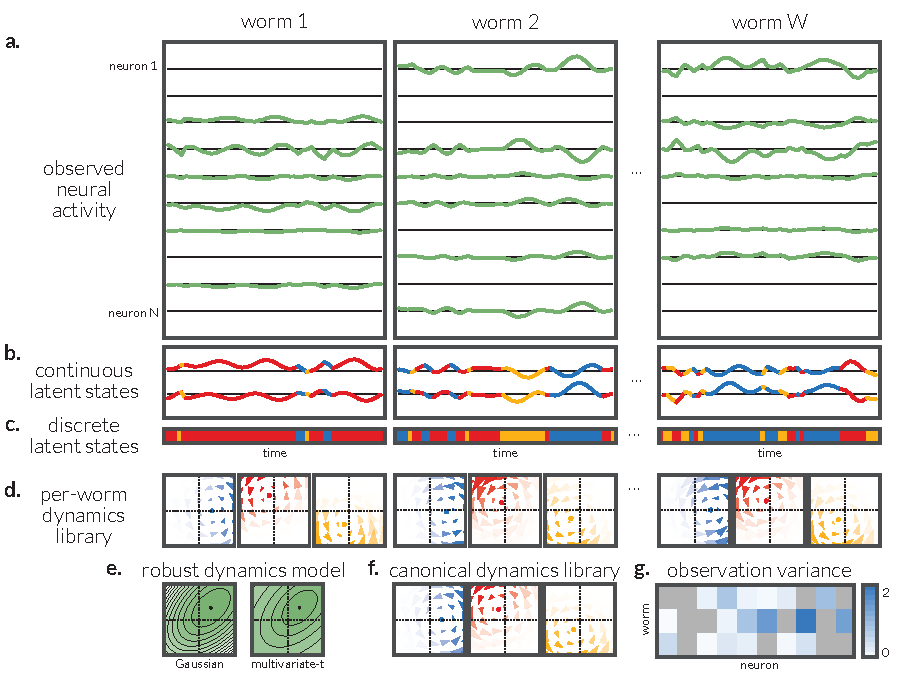
\includegraphics[width=6in]{figures/v3/figure1} 
\caption{
  \textit{A probabilistic framework for combining
  information across multiple worms in order to learn a shared
  dynamical system for \celegans.}
  \textbf{a.}~The data consists of observed neural activity collected
  from many different worms.  In each recording we observe a different
  subset of labeled neurons in the head ganglia.
  \textbf{b.}~We model the observed activity as a linear function of
  an underlying, continuous, and typically low-dimensional latent state,
  here shown as a two-dimensional signal for each recording.
  \textbf{c.}~The dynamics of these continuous states are governed by
  a co-evolving discrete state.
  \textbf{d.}~These discrete states index into a library of linear
  dynamics functions for each worm, here shown as maps from~$\reals^2$ to~$\reals^2$.
  Each dynamics function is selectively used in different regions of
  continuous latent space, as shown by the different intensities of
  the vector field.
  \textbf{e.}~To increase robustness to model misspecification, we
  use a multivariate-t distribution for the noise in the continuous
  state updates.
  \textbf{f.}~Each worm has its own dynamics library, but they are
  constrained to be close to the shared, canonical library.  This
  combines information to learn shared structure while also allowing
  for worm-to-worm variability.
  \textbf{g.} Likewise, we allow each worm to have its own observation
  variances to account for individual differences that may arise from,
  for example, variable levels of fluorescent protein expression.
  Missing neurons are denoted by gray boxes. 
}
\label{fig:model}
\end{figure}

% To model this data, we build on switching linear dynamical systems
% (SLDS) \citep{chang1978state, ackerson1970state, hamilton1990analysis,
%   ghahramani1996switching, murphy1998switching}, a type of state space
% model that views data as a projection of a low-dimensional latent
% state that switches between linear dynamical regimes.  Formally,
% let~$y_t \in \reals^N$ denote the vector of neural activity observed
% at time~$t$.  The expected activity is given by,~$\E[y_t] = g(x_t)$,
% where~$x_t \in \reals^D$ is a continuous latent state
% and~$g: \reals^D \to \reals^N$ is a linear map. We assume~$D \ll N$,
% reflecting the low-dimensional nature of neural activity. SLDS
% simplify the dynamics of the continuous latent states by introducing a
% discrete latent state~$z_t \in \{1, \ldots, K\}$ that indicates the
% current dynamical regime.  Each discrete regime~$k$ is associated with
% a linear map~$f_k: \reals^D \to \reals^D$. The discrete state~$z_t$
% specifies which map to use in order to propagate~$x_t$ to the next
% time step.  Specifically,~$\E[x_{t+1}] = f_{z_t}(x_t)$. By switching
% between different linear dynamical regimes, the SLDS captures highly
% nonlinear dynamics.  We seek to infer the continuous and discrete
% latent states and simultaneously learn the linear maps, the
% distribution of the noise in the observations and the continuous
% states, and the dynamics that govern how the discrete latent states
% evolve.
To model this data, we build on switching linear dynamical systems
(SLDS) \citep{chang1978state, ackerson1970state, hamilton1990analysis,
  ghahramani1996switching, murphy1998switching}, a type of state space
model that views data as a projection of a low-dimensional latent
state that switches between linear dynamical regimes.  The expected
activity is a linear function of an underlying, continuous latent
state, illustrated as two-dimensional time series for each worm in
Fig.~\ref{fig:model}b.  We typically assume this latent state is lower
dimensional than the number of observed neurons. SLDS simplify the
dynamics of the continuous latent states by introducing discrete
latent states that indicate the current dynamical regime
(Fig.~\ref{fig:model}c).  Each discrete regime is associated with a
linear map (Fig.~\ref{fig:model}d), and the discrete state specifies
which map to use in order to propagate the continuous latent state to
the next time step.  By switching between different linear dynamical
regimes, the SLDS captures highly nonlinear dynamics.  We seek to
infer the continuous and discrete latent states and simultaneously
learn the linear maps, the distribution of the noise in the
observations and the continuous states, and the dynamics that govern
how the discrete latent states evolve.

% Recurrent model
Standard SLDS treat the discrete latent states as a simple Markov
process: the next state depends only on the current state. However,
this neglects the more nuanced ways in which discrete and continuous
states may co-evolve. For example, the next discrete state may depend
on both the current discrete state and the current location in
continuous latent space; intuitively, different dynamical regimes may
be employed in different regions of continuous latent space. These
types of dependencies are captured by what are variously called
hybrid~\citep{paoletti2007identification},
augmented~\citep{barber2006expectation}, or \emph{recurrent} state
space models~\citep{linderman2017recurrent}. The maps in
Fig.~\ref{fig:model}d illustrate how these dependencies may modulate
the probability of different dynamics depending on the current
location in continuous latent space. We employ these recurrent models
to learn dynamical regimes that are selectively employed as a
function of current continuous brain state.

% Robust model
While recurrent SLDS can approximate highly nonlinear systems, they
are still misspecified. \emph{Robust} methods~\citep{huber1981robust}
ameliorate this concern by lessening the penalty on observations that
do not quite match the dynamics of the current regime.  We achieve
this robustness by replacing the standard Gaussian noise model with a
multivariate-t distribution~\citep{lange1989robust}.  The heavy tails
of this distribution Fig.~\ref{fig:model}e compares a multivariate-t
distribution to a Gaussian with the same mean; though they have
the same covariance shape, the tails of the robust model fall off
more slowly than those of the Gaussian, allowing for outliers and a
degree of model misspecification. 

% Hierarchical model
The third component of our framework is a \emph{hierarchical} model
for learning canonical dynamics from partial recordings collected from
many worms.  Since each recording contains a different subset of
labeled neurons, our first step is to align the data, treating the
activity of neurons that were not found in a given recording as
missing data that must be inferred.  We handle this by integrating
over possible activity of the missing neurons, analytically
marginalizing out this missing data.  The second challenge is
combining information from many recordings while also allowing for
worm-to-worm differences.  For example, the neural activity may have
larger variance in some recordings than in others due to different
levels of expression of the fluorescent protein.  We allow for this by
having a separate variance for each worm and neuron, as shown in
Fig.~\ref{fig:model}g.  More importantly, the dynamics of neural
activity may be slightly different from worm to worm.  We account for
this by introducing a canonical library of dynamical regimes
(Fig.~\ref{fig:model}f) that are shared by all worms as well as a
unique library for each individual worm (Fig.~\ref{fig:model}d);
however, we constrain the per-worm dynamics to be close to the
canonical dynamics.

% Inference
We fit the the canonical and per-worm dynamics libraries, the
parameters of the dynamics and observation noise models, and the
discrete and continuous latent states with approximate Bayesian
inference as described in the Supplementary Material. Briefly, we
separate the problem into two steps: learning the continuous latent
states and the mapping from continuous latent states to observations,
then learning the dynamics libraries that govern the continuous latent
states and the corresponding discrete state sequences.  Both steps are
performed with a block Gibbs sampler, leveraging the structure of the
probabilistic model to perform efficient conditional updates of the
various parameters. 

\subsection*{Hierarchical state space models smooth noisy recordings and predict missing data}

\begin{figure}[t!]
\centering
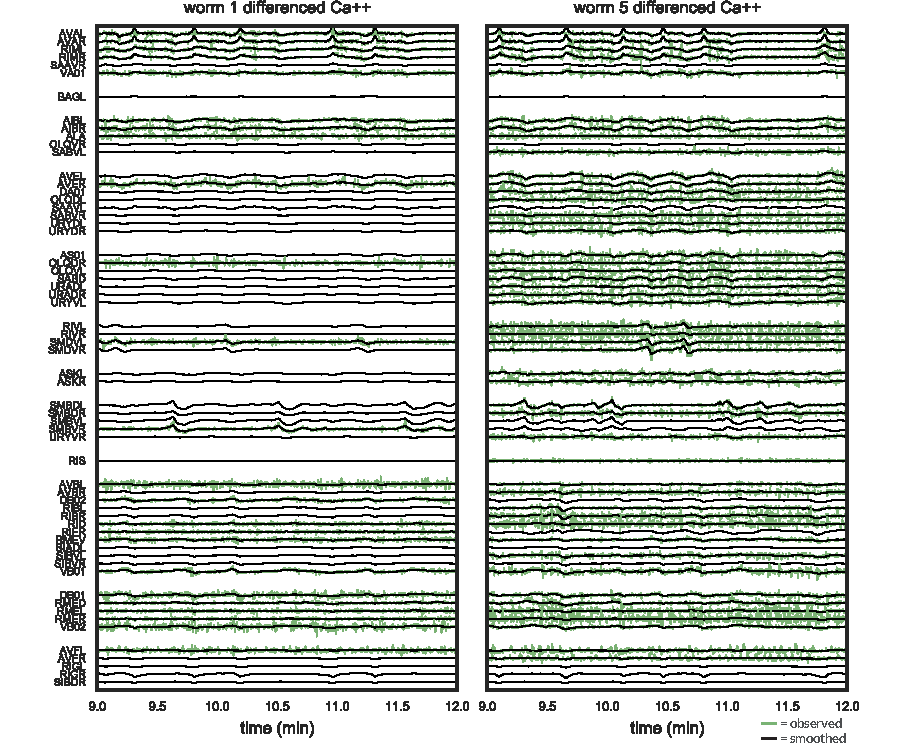
\includegraphics[width=6in]{figures/v3/figure2} 
\caption{ \textit{Hierarchical state space models smooth noisy
    recordings and predict the activity of unseen neurons.}  We show
  the neural activity (differenced Ca++ traces) for two of the
  five worms from the \citet{kato2015global} dataset.  Of these five
  worms, worm 1 (left) has the fewest labeled neurons and worm 5
  (right) has the most.  Green lines are the measured activity of the
  labeled neurons; black lines are the smoothed activities predicted
  by the model for the 61 neurons that were labeled in at least one
  worm.  The model uses correlations learned across all recordings to
  predict the activity of unlabeled neurons, like \textsf{SMBDL} in
  worm 1.  The neurons have been clustered based on similarity, as
  discussed in Fig.~\ref{fig:clustering}.  }
\label{fig:smoothing}
\end{figure}


The parameters of the learned model offer novel insights into the
structure of neural activity in the head ganglia that can only be
obtained by pooling information across many partial recordings.  We
fit our model directly to the first-order differences in calcium
fluorescence; our only preprocessing step is to correct for
photo-bleaching. The green lines in Fig.~\ref{fig:smoothing} show a
three minute window of bleaching-corrected, differenced calcium traces
for two of the five worms in the~\citet{kato2015global} dataset. Of
these five worms, Worm 1 has the fewest labeled neurons (24 neurons)
and worm 5 has the most (48 neurons). Across the five worms, 61 unique
neuron labels were identified in at least one worm.

By aggregating information across worms, the model learns correlation
structure that enables it to smooth noisy traces and predict the
activity of unobserved neurons.  The smoothed and predicted activity
is shown as black lines in Fig.~\ref{fig:smoothing}. For example,
even though \textsf{SMDVR} is not labeled in worm 1, the model
learns how its activity covaries with that of other neurons
by leveraging information from other worms, like worm 5, in which
both~\textsf{SMDVR} and~\textsf{SMDVL} are labeled.  Since these
two neurons are highly correlated, the model can make strong predictions
about the activity of~\textsf{SMDVR} in worm 1 on the basis of the
activity of~\textsf{SMDVL}.

The degree to which the smoothed activity matches the observed
activity is governed by the dimensionality of the latent state space.
We estimate this dimensionality with cross validation, reserving the
last 20\% of the data (3.6 min) for testing and measuring the marginal
log likelihood of the held-out data as we increase the latent
dimensionality. We find that the test likelihood peaks with a
10-dimensional latent state (Fig.~\ref{fig:supp_emissions}c).

Moreover, the likelihood is substantially higher in the model that
includes per-worm observation variances compared to the model with
shared variances for all worms. Fig.~\ref{fig:supp_emissions}d shows
the inferred variance for each worm in the \citet{kato2015global}
dataset.  Neurons that were not identified are marked with a gray box.
This shows the extent of the missing data and the need for
hierarchical modeling.\todo{make supplement figure}
 
\subsection*{Emission model reveals clusters of functionally similar neurons}

\begin{figure}[t!]
\centering
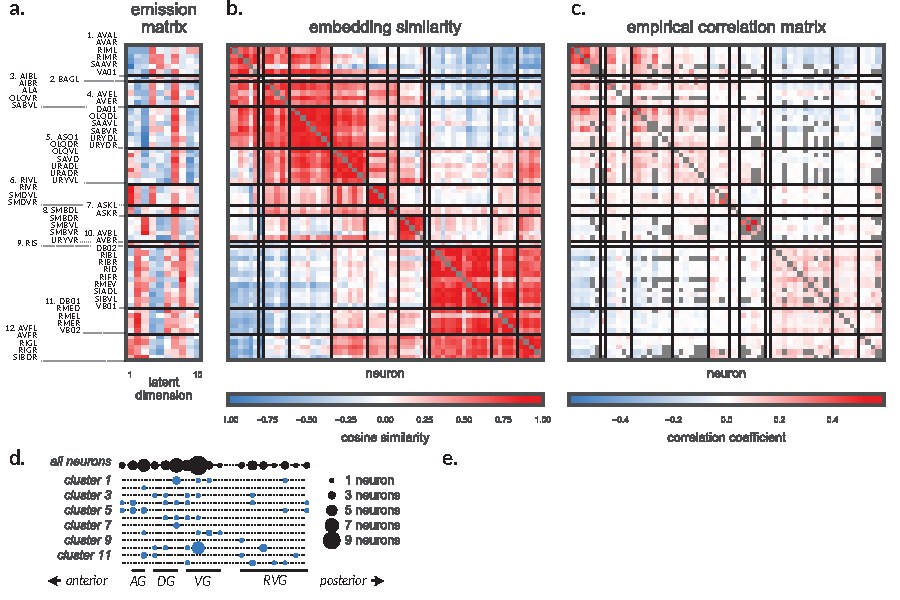
\includegraphics[width=6in]{figures/v3/figure3B} 
\caption{ \textit{The mapping from continuous latent states to neural
    activity reveals clusters of functionally similar neurons.}
  \textbf{a.} The emission matrix is a linear map from latent states;
  the rows can be seen as ``tuning vectors'' that specify how each
  neuron responds to changes in the latent state.  These tuning
  vectors cluster into discrete groups (separated by black lines),
  indicating that there are subpopulations of similarly tuned, and
  hence highly correlated, neurons. Neurons are ordered as in
  Fig.~\ref{fig:smoothing}. \textbf{b.}~The pairwise similarity between
  tuning vectors supports this clustering and shows differences
  between subpopulations (clusters have been sorted to make this as
  close to diagonal as possible).  \textbf{c.}~The tuning similarity
  reflects correlations between neurons, but since it is learned as
  part of a hierarchical model, it predicts similarities for all pairs
  of neurons, even pairs that are never simultaneously recorded (gray,
  off-diagonal boxes).  \textbf{d.}~We show the spatial locations of
  neurons from each cluster, as specified by WormAtlas.  Neurons in
  the same cluster are not necessarily close to one another in space,
  though some clusters are spatially localized. Black bars denote
  approximate locations of the anterior (AG), dorsal (DG), ventral
  (VG) and retrovesicular ganglia.}
\label{fig:clustering}
\end{figure}


The linear mapping from latent states to observations reveals clusters
of similarly tuned neurons.  The mapping is given by a matrix with
rows corresponding to neurons and columns corresponding to latent
dimensions, shown in Fig.~\ref{fig:clustering}a.  Each row can be seen
as a \emph{tuning vector} that specifies how the corresponding neuron
responds to each dimension of the latent state.  This matrix reveals
groups of similarly tuned neurons. To capture this, we used k-means to
cluster the neurons based on their tuning vectors and found that 12
clusters adequately captures the diversity of the population.  Using
fewer clusters leads to qualitatively similar groups but omits some of
the finer within-group differences; allowing more clusters eventually
leads to groups of lateral pairs (like \textsf{ASKL} and \textsf{ASKR}
in a.).  The neurons are ordered as in Fig.~\ref{fig:smoothing}, and
clusters are separated by black lines.

Fig.~\ref{fig:clustering}b shows the cosine similarity of tuning
vectors for each pair of neurons, illustrating the differences
and similarities between clusters.  We notice two prominent
features.  First, the block structure of this
matrix lends support to the notion of discrete clusters, indicating
strong similarity between neurons within the same cluster. Second,
we have sorted the clusters in order to make this matrix as
diagonal as possible.  Upon doing so, we see a banded structure
indicating that in addition to the discrete clustering, there is
also a continuum along which these clusters vary, with the first
clusters more similar to each other than to the latter clusters.
Since the diagonal values equal one by definition, these
have been grayed out. 

In our model, the emission matrix determines the correlations between
neurons.  As such, we expect the similarity between rows of the
emission matrix to mimic the empirical correlations observed in the
data.  Fig.~\ref{fig:clustering}c shows that this is indeed the case,
as neurons with similar tuning vectors also have higher empirical
correlation coefficients.  However, without a hierarchical model, we
cannot empirically estimate the correlation between pairs of neurons
that were not simultaneously observed.  For this dataset, this leaves
many entries in the empirical correlation matrix missing, as denoted
by the gray off-diagonal entries. A key advantage of our hierarchical
model is its ability to draw inferences in the face of significant
amounts of missing data.

What can explain this clustering?  We first look at the spatial
locations of neurons in each cluster, under the hypothesis that
clusters could be trivially explained by an inability to resolve
differences in activity between nearby neurons.
Fig.~\ref{fig:clustering}d shows the locations of all 61 labeled
neurons, using the positions from WormAtlas\todo{cite} along the
head-tail axis of the worm's body.  The size of the dot indicates the
number of neurons at that location; the bars below denote the
approximate location of the anterior (AG), dorsal (DG), ventral (VG)
and retrovesicular (RVG) ganglia.  Some cluster (e.g. cluster 6) are
spatially localized, but many clusters contain neurons from multiple
head ganglia.  This suggests that location alone cannot explain the
similarity between tuning vectors.

\todo[inline]{Break down clustes by type (sensory/inter/motor
  neuron).}

\todo[inline]{Ask Manuel/Annika to label functional role of neurons.}


\subsection*{Model predictions aid in neural identification}

\begin{figure}[t!]
\centering
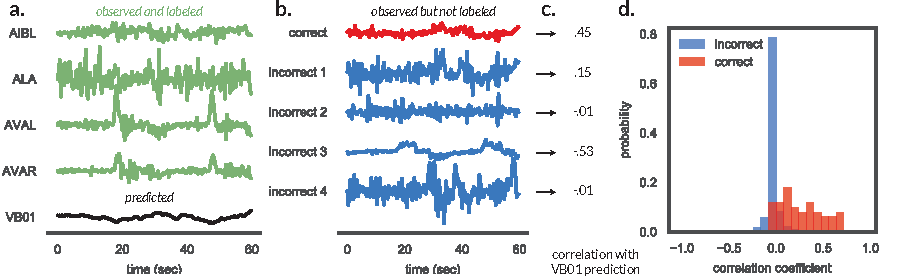
\includegraphics[width=6in]{figures/v3/figure_id} 
\caption{ \textit{The predicted neural activity is a useful aid for
    neural identification.}  \textbf{a.} The model uses observed and
  labeled activity (green traces) to predict the activity of unlabeled
  neurons, as in Fig.~\ref{fig:smoothing}. \textbf{b.} Alongside the
  labeled activity, we also have traces from many neurons that could
  not be unambiguously labeled. To test whether the model's
  predictions could aid in labeling neurons, we conducted a synthetic
  experiment, withholding the activity of some labeled neurons. Here,
  the red trace is the withheld activity of VB01 and the blue traces
  are the activity of other unlabeled neurons.  Together, these make
  up a pool of candidates for the VB01 label.  \textbf{c.} For each
  candidate, we measured the correlation between its activity and the
  predicted activity of VB01.  \textbf{d.} Repeating this experiment
  50 times, we found that the correct candidates tend to be much more
  correlated with the model's predicted activity than the other,
  incorrect candidates.  Thus, the model's predictions serve as a
  useful aid for labeling neurons.  }
\label{fig:id}
\end{figure}

The predicted activity is based on the correlations between neurons
learned from many recordings.  These predictions should be a useful
aid for laneling neurons whose activity could be measured but whose
identity could not be unambiguously resolved.  To test this
hypothesis, we conducted a synthetic experiment in which we withheld
the labels of ten neurons per worm.  We fit the model to the remaining
neurons and then compared the model's predicted activity to the
activity of the heldout neurons, as well as to the activity of the
unlabeled neurons identified by~\citet{kato2015global}.

Fig.~\ref{fig:id}a shows a schematic of the experiment: though VB01
was labeled in the dataset, we withheld its activity and used the
model to predict it (black trace) based on the observations of the
other, labeled neurons (green traces).  We then compared the model
predictions to the true activity of VB01 (red trace) and to the
activity of other neurons that were identified but not labeled (blue
traces), as shown in Fig.~\ref{fig:id}b.  We computed the correlation
coefficient between these traces and the predicted activity of VB01,
as shown in Fig.~\ref{fig:id}c.
We find that in this case, the model's predictions and the true activity
are highly correlated, even though the true activity was not used
when training the model.  We repeated this experiment for 50 heldout
neurons and found that this pattern holds: the predicted activity is
typically much more correlated with the activity of the correct
heldout trace (red histogram) than with the activity of other unlabeled
neurons (blue histogram).  This suggests that our hierarchical model
may serve an additional role in aiding neural identification in
ambiguous, noisy data. 

\todo[inline]{Also discuss simultaneous matching experiments? Possible
  improvements from including more labeled neurons.  Work with Gonzalo
  on learning permutations.  Importance of capturing uncertainty in matching.}


\subsection*{SLDS automatically parse data into discrete, behaviorally meaningful states}

\begin{figure}[t!]
\centering
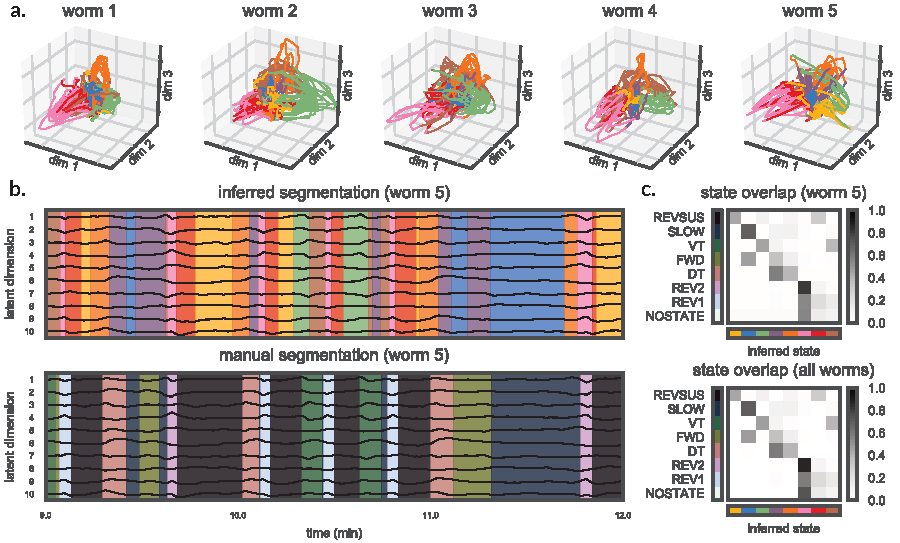
\includegraphics[width=6in]{figures/v3/figure4} 
\caption{ \textit{The hierarchical SLDS automatically segments neural
    activity based on its dynamics.}  \textbf{a.}~The top three
  dimensions of the inferred continuous latent states for each of the
  five worms, color coded by the corresponding discrete latent state.
  \textbf{b.}~The inferred segmentations (top) align with the manual
  segmentations (bottom) of~\citet{kato2015global}, though some
  manually labeled states are split into multiple inferred states
  (e.g. forest green state is often split into green and brown) and
  others are combined (e.g. light purple, light blue, and white are
  often combined into pink).  \textbf{c.}~We quantified the overlap
  between the manual and inferred states and found a close
  correspondence.  As~\citet{kato2015global} showed, the manually
  labeled states map onto different behaviors (\textsf{REVSUS}:
  sustained reversal; \textsf{SLOW}: slow forward crawl; \textsf{VT}:
  ventral turn; \textsf{FWD}: forward crawl; \textsf{DT}: dorsal turn;
  \textsf{REV1, REV2}: reversals; \textsf{NOSTATE}:
  undetermined). The correspondence between inferred and manually
  labeled states implies that hierarchical state space models can
  infer behaviorally meaningful states directly from neural activity.}
\label{fig:syllables}
\end{figure}

Having learned a mapping from latent state space to observed activity,
we can now reason about the dynamics of these continuous latent
states. Fig.~\ref{fig:syllables}a plots the trajectory of the first
worm's neural activity in the top three dimensions of the continuous
state space, color coded by the discrete regime inferred under the
SLDS.  These are the three dimensions with the highest percentage of
expained variance. We see that different regimes correspond to
distinct loops through latent space.  Compare this with Fig. 4b
of~\citet{kato2015global}---they achieved a similar result by manually
segmenting smoothed trajectories in the space spanned by the first
three principal components.  In contrast, our probabilistic framework
is automatic, operates on ten-dimensional latent states, and requires
no additional smoothing.

We use the likelihood of held-out test data to determine
the number of discrete regimes and assess the value of the robust and
recurrent model extensions, as shown in Supplemental Fig.~\ref{fig:modelselection}.
While the non-robust models with Gaussian dynamics noise achieve
higher training likelihood, the robust models generalize better to
test data.  Moreover, the recurrent models provide further improvement
over the standard Markovian models.  We find that test likelihood is
maximized with eight latent states, which matches the number manually
chosen by~\citet{kato2015global}.

Not only does the SLDS find the same number of states, it also finds a
close correspondence between the manually labeled and inferred states.
Fig.~\ref{fig:syllables}b shows ten-dimensional latent states and the
manual and inferred segmentations for a 5.5 minute section of data.
The manual and inferred states often change at similar times. We also
see instances where there appears to be a change in continuous state
dynamics that are identified by the SLDS before it is detected in the
manual segmentation (e.g. around 11.8 min).  Fig.~\ref{fig:syllables}c
quantifies the overlap in states for the first worm and for all worms.
Many inferred states are in one-to-one correspondence with manually
labeled states. Some manual states are split into two inferred states
(e.g. ventral turns (\textsf{VT}) are split into green and brown) and
others are combined (e.g. reversals and undetermined states
(\textsf{REV1}, \textsf{REV2}, \textsf{NOSTATE}) map onto pink).
The correspondence between manual and inferred states shows that
the hierarchical SLDS is a useful tool for automatically segmenting
brain data into behaviorally meaningful states.


\subsection*{Quantifying the dynamics of neural activity in each discrete state}
The hierarchical SLDS not only automates the laborious manual
segmentation process, it justifies its segmentation with a
quantitative definition of each inferred state. Each state is
associated with a set of canonical linear dynamics, as shown in
Fig.~\ref{fig:dynamics}a. The arrows in these vector fields show where
the continuous state is mapped to under the corresponding discrete
state (for the top three latent dimensions).  Arrows are only drawn
at those locations where the discrete state was actually employed.

States 1 (blue), 3 (yellow), and 5 (purple) are all characterized
by convergence toward the origin, which corresponds, essentially, to
no change in neural activity. These three states differ in terms of how
quickly they converge to the origin and the amount of rotation as
they do so.  By contrast, states 2 (red), 4 (green), 6 (orange), 7(brown)
and 8 (pink) form parts of rotational loops in latent state space.
As the latent state traces out a loop, it transiently activates
the clusters of neurons that are tuned to the loop direction.
These states are associated with dorsal turns, ventral turns, and
reversals.

We use these dynamics to simulate how brain activity evolves
under the different states. Fig.~\ref{fig:dynamics}b shows how four
simulated trajectories of each state from various starting locations map 
into activations in the space of neural activity. For each discrete state,
we chose the starting locations randomly from the set of locations where
that state was entered in the real data.  We then simulated forward in
time according to that state's dynamics until the simulation predicted
a state change.  We then mapped these four simulations for each state
through the emission matrix and measured the average activation induced
on each of the 12 neural clusters.

These activations lend further evidence in support of the behavioral
labels attributed to each state. For eaxample, state 4 (green) coincides
with the manually labeled ``ventral turn'' state.  Its dynamics produce
a pronounced rise in the activity of cluster 6, which (referring back
to Fig.~\ref{fig:clustering}), consists of the \textsf{RIVL/R} and
\textsf{SMDVL/R} neurons.  The \textsf{RIV} pair are polymodal inter-
and motor-neurons that specify the ventral bias of turns, and the
\textsf{SMDV} are motor neurons that initiate ventral turns.  State 4
dynamics also tend to suppress the activation of cluster 8, which
consists mostly of the \textsf{SMB*} neurons.  As these neurons are
implicated in dorsal turns, this again makes sense. Finally, we see
that states 6 (orange) and 5 (purple) often produce a rise and fall, respectively,
of activation on cluster 8, which together produce a dorsal turn.
These two states do indeed coincide with the manually labeled dorsal
turn state, again confirming the behavioral interpretation of these
dynamical states.

Finally, Fig.~\ref{fig:dynamics}c shows the eigenspectra of the linear
dynamics for each worm and each state.  Imaginary eigenvalues give
rise to rotational dynamics, and the magnitude of the eigenvalues
determines whether the state is stable or not.  If the magnitude is
greater than one (outside the unit disk denoted by the black arc),
the dynamics produce exponential growth in the latent state space; if
the eigenvalues are all less than unit magnitude, the dynamics converge
to a fixed point.  As expected, the rotational states do indeed have
more imaginary eigenvalues, and most states have eigenvalues with
magnitude near one.  Some states, like the brown state, have eigenvalues
larger than one, which produce unstable dynamics, though this is
somewhat balanced by the recurrent extensions discussed in the next
section.  Comparing across rows, we see only minor differences from worm
to worm, substantiating our hierarchical modeling assumptions.

\begin{figure} [b!]
  \caption{ \textit{(Next page.) Discrete states are characterized by
      simple linear dynamics that give rise to interpretable patterns
      of neural activity.}  \textbf{a.}~Each discrete state is
    associated with a canonical set of linear dynamics, which can be
    viewed as mappings from~$\reals^{10}$ to~$\reals^{10}$.  We show
    the mappings for the first three dimensions here, with vectors
    placed at locations where each state was used.  \textbf{b.}~We
    simulated four latent state trajectories with these linear
    dynamics from different starting locations, and then we mapped
    these latent state trajectories through the emission matrix to
    compute a time course of resulting activations for each cluster of
    neurons.  \textbf{c.}~The eigenspectra of the dynamics matrices
    provide insight into the nature of the states: imaginary eigenvalues
    give rise to rotational dynamics and the magnitude determines
    whether the stability of the dynamics. The arc denotes
    the unit magnitude line; eigenvalues to the left are contractive
    and to the right are expansive. Looking across rows, we
    see how the spectra vary from worm to worm. }
\end{figure}
\addtocounter{figure}{-1}

\begin{figure}[h!]
  \centering
  \vspace{-.5in}
  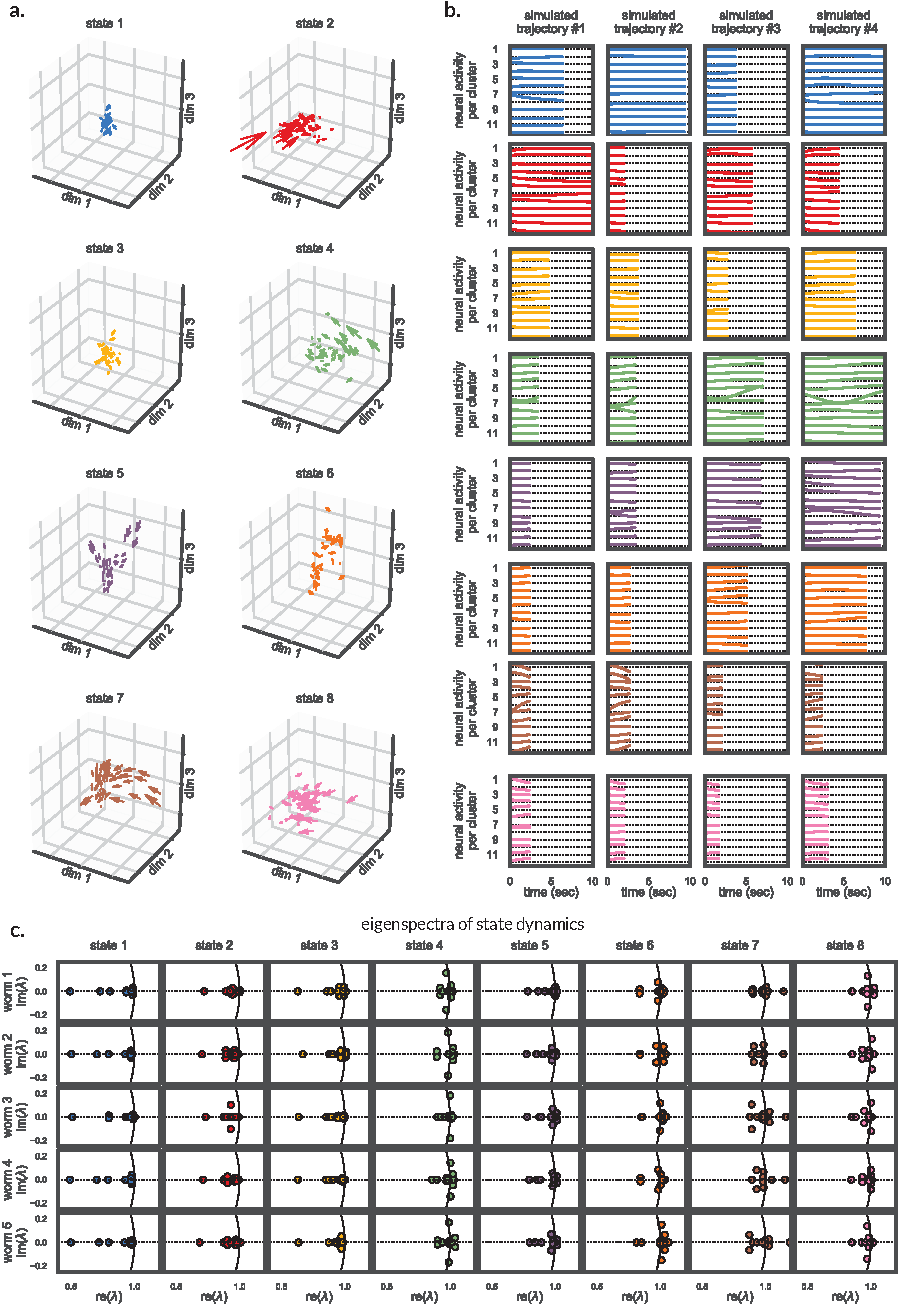
\includegraphics[width=6in]{figures/v3/figure5B}
  \caption{Caption on preceding page.}
  \label{fig:dynamics}
\end{figure}

\clearpage

\subsection*{Recurrent models learn spatially localized states and non-Markovian dynamics}

\begin{figure}[t!]
\centering
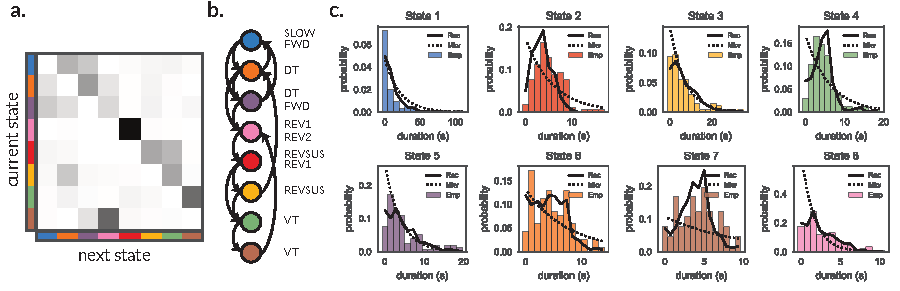
\includegraphics[width=6in]{figures/v3/figure6} 
\caption{ \textit{Discrete state transitions show a chain-like structure
    with non-Markovian durations.}  \textbf{a.}~Counts of inferred transitions
  from one state to another. The states are permuted to emphasize the
  feed-forward structure.  \textbf{b.}~An alternative view of the
  transitions; each state is a node in a graph and edges denote
  high-probability transitions.  This shows transitions between
  forward and reverse crawling linked by dorsal and ventral turns.
  \textbf{c.}~The standard SLDS assumes Markovian transitions, which
  imply a geometric distribution of state durations (dotted black
  lines), but Fig.~\ref{fig:syllables} suggests that state
  transitions occur near the origin.  With the exception of state 7,
  which is unstable, the recurrent SLDS incorporates
  this dependency and generates state durations (solid black lines)
  that are a better fit to those inferred from the data (colored
  bars).  }
\label{fig:recurrent}
\end{figure}

The final component of our hierarchical state space model is the
discrete transition distribution.  In contrast to standard SLDS, we
allow these transition probabilities to depend on the location in
continuous state space (via the \emph{recurrent} dependency) as well as
the preceding discrete state (the \emph{Markovian} dependency).
Fig.~\ref{fig:recurrent}a shows the contribution of the Markovian
term.  Each cell in this matrix denotes the number of transitions from
one state to another. We are only counting transitions in which the
state changes, hence the diagonal is zero.  We have permuted the
states to emphasize the largely feed-forward structure.

Fig.~\ref{fig:recurrent}b shows the strongest entries in this matrix
in an alternative form.  We have illustrated each state as a node in a
graph, and labeled the states based on their correspondence with the
manually labeled states of~\citet{kato2015global} (see
Fig.~\ref{fig:syllables}d).  This reveals a chain-like transition
structure in which slow and forward (\textsf{FWD}) crawling are linked
to reverse (\textsf{REV1}, \textsf{REV2}) and sustained reverse
(\textsf{REVSUS}) via dorsal turns (\textsf{DT}). From sustained
reverse crawling, the worm may execute either dorsal or ventral turns
(\textsf{VT}).

To accurately model these dynamics, the changes must occur at precise
locations in continuous latent space.  Namely,
Fig.~\ref{fig:syllables}a shows that the loops tend to start and end
at the origin, and we rarely see transitions when the continuous
latent state is far from zero. This manifests in signature duration
distributions for the various states.  Fig.~\ref{fig:recurrent}c plots
these distributions for each of the eight states.  Superimposed on
top, we show the predicted distributions with the recurrent SLDS
(solid black lines) compared with the predictions of the standard,
Markovian SLDS (dotted black lines). The Markovian model knows nothing
of the continuous latent state and implies a geometric duration
distribution with monotonically decreasing probability. By contrast,
the recurrent model learns to transition near the origin, which
gives rise to characteristic duration distributions that closely
match the empirical distributions. 


\subsection*{Oxygen level modulates transition probabilities but not dynamics or emissions}

\begin{figure}[t!]
\centering
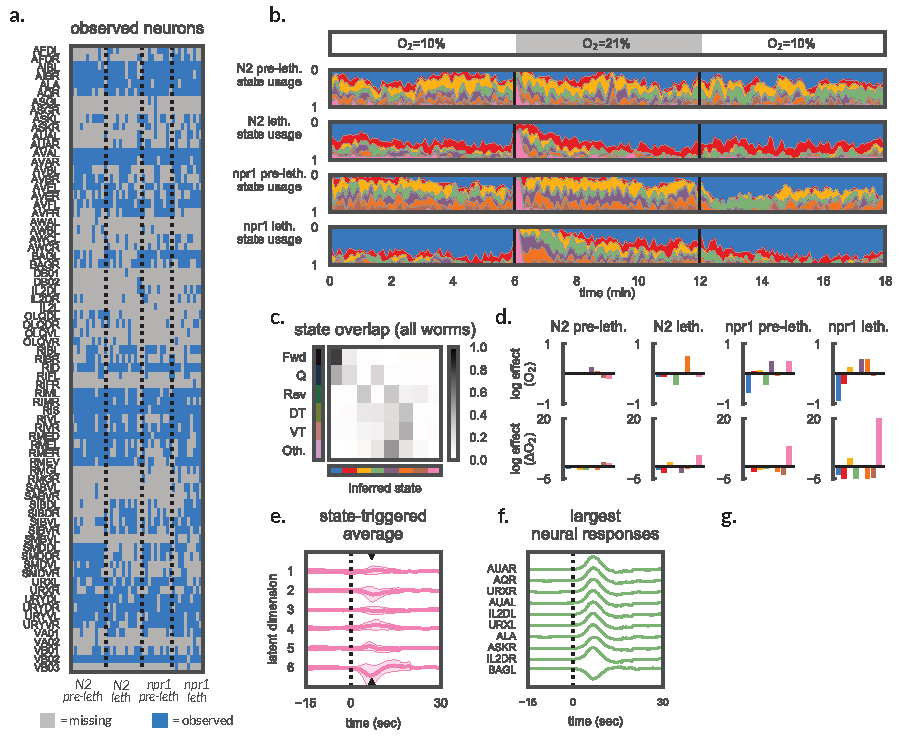
\includegraphics[width=6in]{figures/v3/figure7} 
\caption{\textit{Incorporating exogenous factors like oxygen level
    into the dynamics model yield differential responses in worms from
    different genetic strains and developmental stages.}
  \textbf{a.}~The observed neurons variances for each of the 41 worms
  in the~\citet{nichols2017global} dataset.  \textbf{b.}~Worms of
  different genetic strains (N2, npr1) and developmental stages
  (pre-lethargus, lethargus) exhibit different average state usages as
  a function of the oxygen level.  Blue and red states are much more
  likely in the lethargus stage for both genetic strains, but they are
  suppressed in npr1 worms at high oxygen concentrations. Moreover, we
  see a pronounced increase in the pink state usage immediately after
  the oxygen level increases to 21\%.  \textbf{c.}~As above, the
  inferred states closely match the manually labeled states
  of~\citet{nichols2017global}, with blue, red, and to a lesser extent
  green mapping onto the forward (\textsf{Fwd}) and quiescent
  (\textsf{Q}) states.  \textbf{d.}~We extended the model to
  incorporate oxygen level (O$_2$) and change in oxygen level
  ($\Delta$O$_2$) as exogenous factors that drive discrete transition
  probabilities.  We find that oxygen level has a limited effect on N2
  worms but strongly suppresses the blue (\textsf{FWD/Q}) state in
  npr1 worms and promotes the purple and orange
  (\textsf{Rev/DT/VT/Other}) states. The largest effect arises from
  the change in oxygen: an increase in $O_2$ strongly elicits the pink
  state.  \textbf{e.} The state-triggered average latent state
  trajectory following entry into the pink state shows a dip in
  activity along the last dimension 7 seconds after entry (black
  arrows).  \textbf{f.} This dip gives rise to strong opposing
  responses of sensory neurons \textsf{URXL/R} and \textsf{BAGL}
  (among others), which are known to respond to increases and
  decreases, respectively, in oxygen concentration.  }
\label{fig:o2}
\end{figure}

The preceding results demonstrated the efficacy of hierarchical,
recurrent, and robust SLDS for learning interpretable dynamics of
neural activity from the noisy, partial recordings
of~\citet{kato2015global}.  We now turn to the dataset studied
in~\citet{nichols2017global}, which contains many more worms with
roughly the same number of neurons per recording but is complicated by
additional factors.  First, there are two strains of worms (N2 and
npr-1) at two different stages of development (pre-lethargus and
lethargus); second, the oxygen level is manipulated over the course of
the recordings to elicit different responses.  Here we show how our
framework can be extended to study the effects of these manipulations.

Fig.~\ref{fig:o2}a shows which neurons were labeled in each of the
recordings along with the inferred observation variance. There are 41
worms, roughly ten from each strain and developmental stage
combination (N2 + pre-lethargus, N2 + lethargus, npr1 + pre-lethargus,
and npr1 + lethargus). Some neurons are consistently identified in
almost all worms; others are identified in only a handful.  As before,
our hierarchical framework combines all this information.

Upon fitting our model, we immediately see a difference in the average
usage of the eight states  as a function of oxygen level(Fig.~\ref{fig:o2}b). The worms in the
lethargus stage predominantly use the blue and red states.  Again,
we found a close correspondence between our inferred states and the
manually labeled states of~\citet{nichols2017global}
(Fig.~\ref{fig:o2}c). Here, blue and red both map strongly onto the
quiescent (\textsf{Q}) state. This is consistent with the
characterization of the lethargus stage---at this stage, worms exhibit
much less crawling behavior. The pre-lethargus worms execute a broader
variety of behaviors, including reversals (\textsf{Rev.}) and dorsal
and ventral turns  (\textsf{DT} and \textsf{VT}, respectively). 

A key finding of~\citet{nichols2017global} was that increasing the
oxygen level can elicit activity in lethargus npr1 worms but not in
lethargus N2 worms. We can quantify this effect with our models by
including oxygen level (O$_2$) and change in oxygen level ($\Delta$O$_2$)
as exogenous inputs.
% Fig.~\ref{fig:o2}d
% shows how the graphical model of the recurrent SLDS changes: now the
% discrete state at time~$t$ (red circle) depends on the preceding discrete
% state, the preceding continuous state, and the current oxygen level.
% \todo[inline]{consider alternative models in which oxygen level
%   influences continuous states and observations?}
Fig.~\ref{fig:o2}d (top) shows the inferred effect of oxygen level for each
of the four strain/developmental stage pairs.  As predicted,
higher oxygen levels increase the probability of reversals and
turning related states (orange, purple) and decrease the probability
of forward and quiescent (blue, red, green) states in npr1 worms, but
has limited effect on N2 worms. We do see an increase in turning related
states (orange) in the N2 lethargus worms, but inspection of panel b
indicates this state is still used very sparingly.  Somewhat
surprisingly, the magnitude of the effect is comparable for both
pre-lethargus and lethargus npr1 worms, even though the baseline level
of reversals and turns is much higher in the pre-lethargus worms.

The largest effect is in response to the change in oxygen level, as
shown in Fig.~\ref{fig:o2}d (bottom).  Across all worms, the change
from 10\% to 21\% oxygen concentration sharply increases the probability
of transitioning into the pink state. Moreover, this state is seldom
used except for when the oxygen level increases.  This suggests that
sharp increases in oxygen level induce a transient and characteristic
neural response that is not seen in steady-state oxygen levels.

Fig.~\ref{fig:o2}e shows the average latent state trajectory triggered
upon entry into the pink state (for this dataset, the optimal performance
was achieved by a 6-dimensional state space model).  We see a dip and
rebound along the last dimension approximately 7 seconds after entry
(denoted by the black arrows).  We identified the neurons that showed
the largest response at this point in time and plotted the top ten
in Fig.~\ref{fig:o2}f.  Unsurprisingly, these neurons are largely sensory
and interneurons.  In particular, \textsf{URXL/R} and \textsf{BAGL/R} are
known to jointly encode changes in oxygen level with opposing signs: \textsf{URXL/R}
respond to increases in oxygen, \textsf{BAGL/R} respond to dcreases.  Our
model recapitulates these results and suggests that many other sensory
neurons respond similarly to this stimulus.

\clearpage

\section*{Discussion}

\clearpage

\bibliography{refs}
\bibliographystyle{abbrvnat}

\clearpage

\appendix

\section{Data}
\label{sec:data}

The data comes in the form of a collection of matrices~$\{\widetilde{Y}^{(w)}\}_{w=1}^W$
for each of~$W$ worms.  The matrix~${\widetilde{Y}^{(w)} \in \reals^{T_w \times N_w}}$
represents the calcium activity of the~$w$-th worm, which consists of~$T_w$
time frames and~$N_w$ neurons.\footnote{Technically, this calcium activity is
a matrix of first-order temporal differences of a
bleaching-corrected~$\Delta F /F$ signal. Unlike~\citet{kato2015global}, we
do not smooth these derivatives. We work with the raw first-order
temporal differences.}  \celegans~is special in that each neuron has a unique
name.  Assigning names to neurons in calcium imaging data is a challenging
task, but typically, out of the~${\sim 100}$ neurons observed in any worm,
we can label about~$20-30$ with high certainty.  As such, we choose to
represent each matrix~$\widetilde{Y}^{(w)}$ in \emph{canonical form} as a
tuple~$(Y^{(w)}, M^{(w)})$, where~${Y^{(w)} \in \reals^{T_w \times N}}$ is
a matrix where each column corresponds to one of the~$N$ neurons that is
identified in at least one of the~$W$ worms, and~${M^{(w)} \in \{0,1\}^{T_w \times N}}$
is a corresponding \emph{mask} matrix that indicates which neurons were
observed in worm~$w$.  If~$M_{:,n}^{(w)} = 1$, neuron~$n$ was labeled in
worm~$w$ and~$Y_{:,n}^{(w)}$ was its observed activity.  If~$M_{:,n}^{(w)}=0$,
this neuron was not observed in worm~$w$, and the corresponding activity
is missing.\footnote{The mask is defined in such a way that neurons can
  be missing for only subsets of time frames, but in our data neurons are
  either labeled or missing.}
% todo: note that we could also (and have also) model the activity of
% unlabeled neurons.  For the final analyses, I'm not doing this though.

\section{Hierarchical Generative Model}

We model the neural activity with a switching linear
dynamical system (SLDS) with three new extensions: (i)~a \emph{hierarchical} model
to share parameters across worms while also allowing for worm-to-worm
variability; (ii)~a \emph{robust} model for dynamics noise to help address
model misspecification; and (iii)~a \emph{recurrent} model to capture
how continuous latent states influence discrete state transition probabilities.
We will introduce the SLDS first and then present each of these extensions
in turn.


\subsection{Switching linear dynamical systems}
\label{sec:slds}
Switching linear dynamical system models (SLDS) break down complex, nonlinear
time series data into sequences of simpler, reused dynamical modes.
By fitting an SLDS to data, we not only learn a flexible nonlinear generative
model, but also learn to parse data sequences into coherent discrete units.

The generative model is as follows. At each time ${t=1,2,\ldots,T}$,
for each worm~$w$,
there is a discrete latent state ${z_t^{(w)} \in \{1,2, \ldots,K\}}$ that
follows Markovian dynamics,
\begin{equation}
  z_{t+1}^{(w)} \given z_t^{(w)}, \{\pi_k\}_{k=1}^K  \sim \pi_{z_t^{(w)}}
  \label{eq:markov_z}
\end{equation}
where ${\{\pi_k\}_{k=1}^K}$ is the Markov transition matrix and
${\pi_k \in [0,1]^K}$ is its $k$th row. 
In addition, a continuous latent state ${x_t^{(w)} \in \reals^D}$ follows
conditionally linear (or affine) dynamics, where the discrete state $z_t^{(w)}$
determines the linear dynamical system used at time $t$:
\begin{align}
  x_{t+1}^{(w)} &= A_{z_{t+1}^{(w)}} x_{t}^{(w)} + b_{z_{t+1}^{(w)}} +  u_t^{(w)},
  &
  u_t^{(w)} &\iid\sim \cN(0,Q_{z_{t+1}^{(w)}}),
  \label{eq:slds_start}
\end{align}
for matrices ${A_k, Q_k \in \reals^{D \times D}}$ and vectors~${b_k\in
\reals^D}$ for~${k=1,2,\ldots,K}$.
Finally, at each time $t$ a linear Gaussian observation $y_t^{(w)} \in \reals^N$
(some entries of~$y_t^{(w)}$ are masked off; recall Section~\ref{sec:data}) is
generated from the corresponding latent continuous state,
\begin{align}
  y_t^{(w)} &= C x_t^{(w)} + d + v_t^{(w)}, & v_t^{(w)} &\iid\sim \cN(0,S),
    \label{eq:slds_end}
\end{align}
for $C \in \reals^{N \times D}$, $S \in \reals^{N \times N}$,
and~$d \in \reals^N$. We denote the rows of~$C$ by vectors~$c_n$.
For simplicity, we assume~$C$,~$d$, and~$S$ to
be shared among all discrete states in our model.  Moreover, we assume
the observation noise is diagonal,
\begin{align*}
  S &= \diag\left(\left[s_{1}, \ldots, s_{N} \right] \right). 
\end{align*}
The system parameters comprise the discrete Markov transition matrix, the
library of linear dynamical system matrices, and the neuron-specific
emission parameters, which we write as
\begin{equation*}
  \theta = \{(\pi_k, A_k, Q_k, b_k)\}_{k=1}^K \cup \{c_n, d_n, s_n\}_{n=1}^N.
\end{equation*}

To learn an SLDS using Bayesian inference, we place conjugate Dirichlet priors
on each row of the transition matrix and conjugate matrix normal
inverse Wishart (MNIW) priors on the linear dynamical system parameters,
Gaussian priors on the rows of the emission matrix,
and inverse gamma priors on the emission noise.
We write this as,
\begin{align*}
  \pi_k &\given \alpha \iid\sim \distDirichlet(\alpha),
  &
  [A_k, b_k], Q_k &\given \lambda \iid\sim \distMNIW(\lambda),
  \\
  [c_n, d_n] &\given \eta \iid\sim \distNormal(\eta),
  &
  s_{n} &\given \eta \iid\sim \mathrm{IG}(\eta).
\end{align*}
where~$[\cdot, \cdot]$ denotes column concatenation, and $\alpha$, $\lambda$,
and~$\eta$ denote appropriate hyperparameters of the transitions, dynamics, and
emissions, respectively.


\end{document}
